\section{Results}

\begin{figure*}[h]
    \centering
    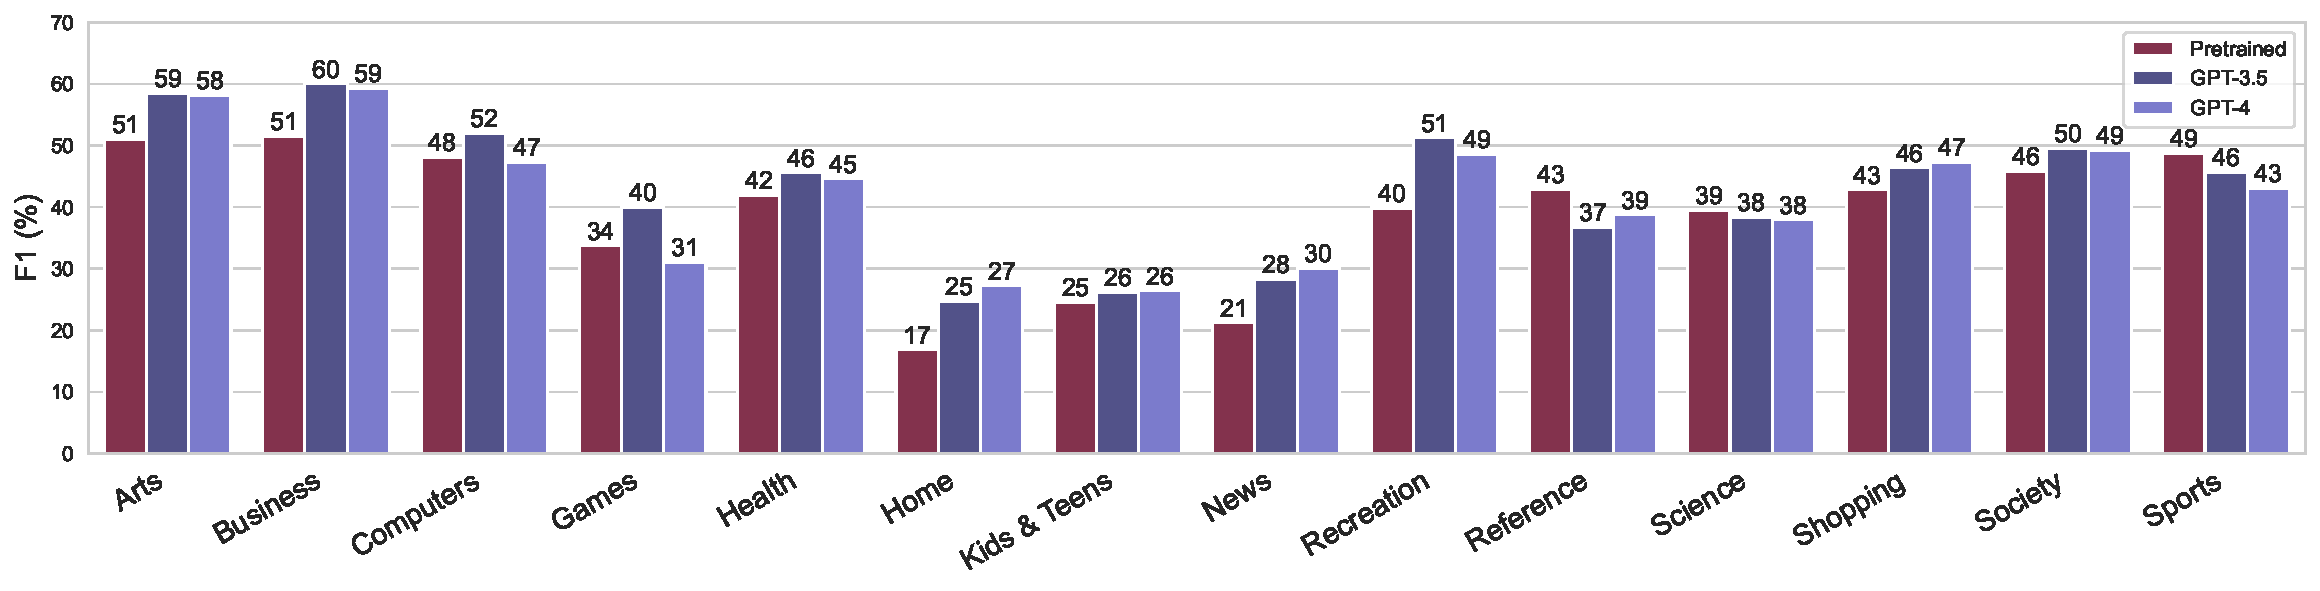
\includegraphics[width=1\textwidth]{./figures/finetune-results.pdf}
    \caption{\textbf{Finetune Results.} Class-wise F1 score for the pre-trained model and the finetuned model on te original crowdsourced data.}
    \label{fig:finetune-results}
\end{figure*}


\subsection*{Phase 1: Identifying an Optimal LLM Labeler}

Table~\ref{tab:labeler-results} shows the results of re-labelling the \texttt{crowdsourced} dataset. Our findings demonstrate that LLM labelers can provide \textit{cost-effective}, and \textit{high-quality} annotations for the complex task of multilingual, multilabel website topic classification. 

% Cost
The labeling cost for the \texttt{crowdsourced} corpus was around \$130 per 1,000 pages. By employing GPT-3.5 and GPT-4 labelers, we reduced the expense to merely \$0.54 and \$6.44 on average respectively, achieving cost reductions of 240x and 20x.

% Calculations
% Human annotator cost: 327 USD
% Pages annotated: 840 * 3 = 2520
% Cost per 1k page: 1000 * 327 / 2520 = 130$

% GPT-3.5 labler cost/1k pages:
% (0.36 + 0.48 + 0.42 + 0.63 + 0.57 + 0.80) / 6 = 0.54

% GPT-4 labler cost/1k pages:
% (4.68 + 5.75 + 5.26 + 7.25 + 6.68 + 8.99) / 6 = 6.44

% Cost reductions:
% GPT-3.5: 130 / 0.54 = 240x
% GPT-4: 130 / 6.44 = 20x

% Performance & Effect of Parameters
The best labeler, GPT-4 with \texttt{context3} and \texttt{1-shot}, achieves a macro F1 score of 46\% compared to the human annotations on the same dataset. It is therefore a better website classifier than the baseline Homepage2Vec model, which achieves a macro F1 score of 39\% on the same dataset. This improvement gives us reason to believe that Homepage2Vec can learn from knowledge of the LLM labelers - the goal of the second phase of our study.

We find that label quality improves with increased information (context and few-shot examples) and model complexity, as shown in Figure~\ref{fig:labelers-grid}. A notable enhancement in label quality occurs when upgrading from \texttt{context1} to \texttt{context2}, and from GPT-3.5 to GPT-4. However, adding sentences and links in \texttt{context3} yields only minor improvements. This implies that solely using the domain and meta-tags in \texttt{context1} is insufficient for accurate topic prediction. Moreover, except for GPT-3.5 in \texttt{context1}, few-shot examples have limited impact on most labelers, suggesting that the task is sufficiently clear from the system prompt and website context.

The range of labels assigned by annotators spans from 0.4 to 2.8. Models are reluctant to assign multiple topics to websites when provided with limited context. However, as more website information becomes available, the number of labels increases, aligning the annotations more closely with those made by humans, who had full website access during their annotation.

\begin{table}[!ht]
\centering
\caption{\textbf{Labeler Statistics}}
\label{tab:labeler-results}
\begin{tabular}{lllccc}
\toprule
 &  &  &  \textbf{LPP} & \textbf{Cost} & \textbf{M.-F1} \\
\textbf{Model} & \textbf{Context} & \textbf{Shot} & ($\mu\pm\sigma$) & (\$) & (\%) \\
\midrule
\multirow[c]{6}{*}{
    \rotatebox[origin=c]{90}{GPT-3.5}
    } & \multirow[c]{2}{*}{\texttt{context1}} & 0-shot & 0.39 ± 0.61 & \textbf{0.36} & 15.96 \\
 &  & 1-shot & 0.91 ± 0.95 & 0.48 & 23.26 \\
 & \multirow[c]{2}{*}{\texttt{context2}} & 0-shot & 1.39 ± 0.98 & 0.42 & 37.59 \\
 &  & 1-shot & 1.68 ± 1.15 & 0.63 & 38.69 \\
 & \multirow[c]{2}{*}{\texttt{context3}} & 0-shot & 1.57 ± 1.08 & 0.57 & 37.24 \\
 &  & 1-shot & 1.85 ± 1.24 & 0.80 & 37.70 \\
\midrule
\multirow[c]{6}{*}{
    \rotatebox[origin=c]{90}{GPT-4}
    } & \multirow[c]{2}{*}{\texttt{context1}} & 0-shot & 1.50 ± 0.93 & 4.68 & 35.55 \\
 &  & 1-shot & 1.83 ± 1.36 & 5.75 & 36.10 \\
 & \multirow[c]{2}{*}{\texttt{context2}} & 0-shot & 2.16 ± 1.03 & 5.26 & 45.39 \\
 &  & 1-shot & 2.49 ± 1.28 & 7.25 & 45.93 \\
 & \multirow[c]{2}{*}{\texttt{context3}} & 0-shot & 2.30 ± 1.11 & 6.68 & 44.10 \\
 &  & 1-shot & 2.80 ± 1.30 & 8.99 & \textbf{46.12} \\
\bottomrule
\end{tabular}
\end{table}



% Cost-quality trade-of
\textbf{Curlie-10k Dataset.} Our analysis reveals a positve trend between label quality and cost, attributable to the use of longer prompts or more sophisticated models. In the next phase, we aimed to select two labelers, one per model. In case of marginal improvements in label quality, we opted for the cheaper labeler. 
The best balance was achieved using \texttt{context2}; the GPT-3.5 labeler employed \texttt{1-shot}, whereas the GPT-4 used \texttt{0-shot}. The average number of topics assigned to a page by the GPT 3.5 labeler is \textbf{1.6} and \textbf{2.03} for the GPT-4 labeler, which is both significantly more than \textbf{1.07} for the original Curlie dataset. Figure~\ref{fig:curlie-10k-dist} shows the distribution of the labels in the re-labelled dataset compared to the original. We can see that, as hoped, more topics are assigned to each page. Interesting differences in the GPT-3.5 and GPT-4 labelers are visible: the GPT-4 labeler tends to assign more websites to the topics that are less frequent in the original dataset, such as \textit{References}, \textit{Kids \& Teens} and \textit{Games}, leading to a more balanced distribution of topics. Surprisingly, the category \textit{Recreation} is assigned to a disproportionally high number of websites by the GPT-4 labeler.

\begin{figure}[!ht]
    \centering
    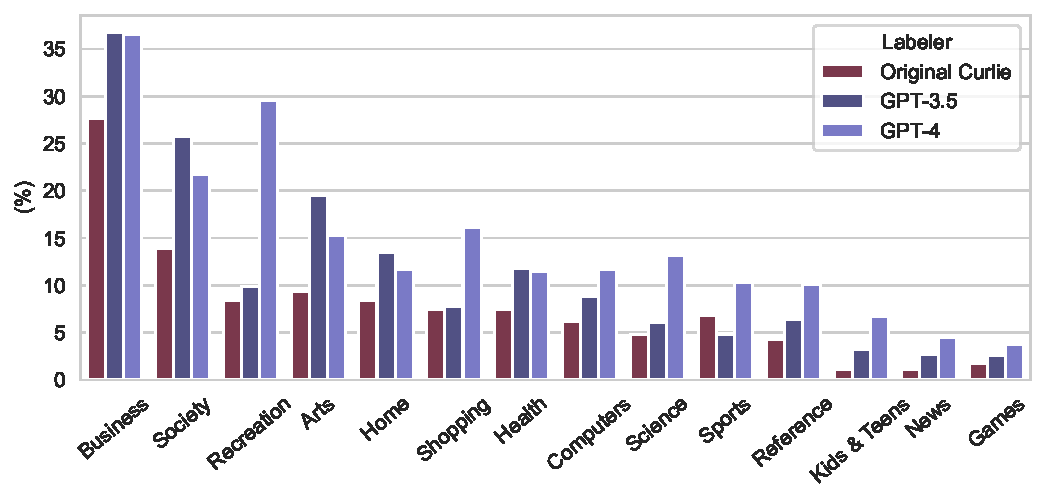
\includegraphics[width=.8\columnwidth]{figures/curlie-10k-dist.pdf}
    \caption{\textbf{Curlie-10k Label Distribution.} Topic distribution of \texttt{curlie-gpt3.5-10k}, \texttt{curlie-gpt4-10k}, as well as \texttt{curlie} for reference.}
    \label{fig:curlie-10k-dist}
\end{figure}

\subsection*{Phase 2: Transferring Knowledge via Finetuning}

% GPT-3.5: 
% LR/ Weight Decay / Scheduler Factor/ Batch Size
% 0.000016	0.064037	0.376673	64
% 1.6e-05 / 6.40e-02 / 3.77e-01 / 64

% GPT 4:
% 0.001535	0.000252	0.460896	64
% 1.5e-03 / 2.52e-04 / 4.61e-01 / 64

Table~\ref{tab:finetune-results} shows the results of the finetuning experiments. We report only the results for the model with the hyperparameter configuration with the best validation macro F1 score. The best hyperparameters are listed in the Appendix~\ref{app:hyperparameters} section. We observe that both models increase the recall from 39.4\% to 51.1\% and 46.4\% when finetuned on GPT-3.5 and GPT-4 labels, respectively. Overall, the macro F1 score increases from 39.2\% to 43.5\% and 43.1\% - an improvement of 4.3 and 3.9 percentage points, respectively.
This improvement shows that we were able to transfer the superior labeling capabilities of the LLM to Homepage2Vec. Figure~\ref{fig:finetune-results} shows that the increase in macro F1 score is achieved consistently acrosss the classes, with 12 out of the 14 classes improving for both models.

% 0.391610 = 39.2% (Pre-trained Homepage2Vec)
% 0.426289 = 42.6% (GPT-3.5) (+3.4 percentage points)
% 0.428    = 42.8% (GPT-4) (+3.6 percentage points)

\begin{table}[!ht]
\centering
\caption{\textbf{Finetuning Results.} The table shows the precision, recall, macro F1 and and labels per page when evaluated on \texttt{crowdsourced}. We show results for the pre-trained baseline, as well as both finetuned variants.}
\label{tab:finetune-results}
\begin{tabular}{lrrrr}
\toprule
 & \textbf{Pr.} & \textbf{Re.} & \textbf{M.-F1} & \textbf{LPP} \\
 & (\%) & (\%) & (\%) & ($\mu$) \\
\midrule
Pretrained & \textbf{40.97} & 39.44 & 39.16 & 1.84 \\
GPT-3.5 & 40.19 & 47.55 & 42.63 & 1.93 \\
GPT-4 & 39.92 & \textbf{49.07} & \textbf{42.87} & \textbf{3.07} \\
\bottomrule
\end{tabular}
\end{table}


